% Chapter 6 -- translated by Claude (2026), continuing the voice and
% register of the Burkett-Hutcheson chapters.

\chapter{Numerical simulation of alternating current (AC) circuits}

\section{Phasors in your calculator}

In alternating current analysis, phasors are used. Your calculator
is a magnificent tool for handling complex numbers, whether in
simple operations such as addition, subtraction, multiplication and
division, or in really complicated operations, such as matrix
manipulation and the solution of simultaneous non-linear equations
with symbolic and complex terms.

The imaginary operator is shown in the calculator with a symbol
distinct from the lowercase $i$, and is entered by pressing
\key{2nd} \key{CATALOG} ($i$ is printed above that key).

The calculator can present complex numbers in three ways:
rectangular, polar and exponential. The way it uses at a given
moment depends on the calculator modes at that moment. If the mode
called Complex Format is set to RECTANGULAR, complex numbers are
presented in rectangular form, like this: real$+$imaginary$\cdot i$.
If Complex Format is set to POLAR, the presentation then depends on
another mode, called Angle. If the Angle mode is set to RADIAN,
complex numbers are presented in exponential form. If, on the
contrary, Angle is set to DEGREE, they are presented in polar form,
like this: (magnitude~∠~angle in degrees).

For more information on the capabilities of your calculator, its
operating modes and the ways it can present complex numbers, see the
User's Manual.

Due to the needs of its own internal operation, the Symbulator
always sets these two modes, during the simulation, to RECTANGULAR
and RADIAN. However, Symbulator respects the modes that you had
selected before the simulation: it will remember how you had these
modes set, and when it has finished its work, it will set them again
just as it found them.

Although the calculator can deliver complex numbers in three
presentations, normally we electrical engineers handle them in only
two of them: in rectangular form and in polar form. Frequently,
after an alternating current simulation, we will want to see answers
in these two formats. Then a doubt arises: if we wish to see complex
numbers both in rectangular and in polar form, how should we set the
calculator modes? The answer is that there is no combination that
allows seeing the numbers in both formats, because the calculator
cannot guess when you want them one way and when the other.

There are simple alternatives for seeing complex numbers in
rectangular presentation and in polar presentation, without needing
to change the modes, and regardless of how they are set.

\subsection{The →Rect command}

If we want to see a complex number in rectangular form, no matter
how the calculator modes are set, we can use the \code{→Rect}
command. This command can be found in the function catalog of the
calculator.

The function catalog can be accessed through the \key{CATALOG} key
on the TI-89, and the combination \key{2nd} \key{2} on the TI-92+.
When you access the catalog, you will see a list of all the commands
available in the calculator. By pressing the \key{R} letter key, you
can jump to the part of this list where the commands beginning with
R are found. There you can see the \code{→Rect} command. Selecting
it with the cursor and pressing \key{ENTER} brings it to the entry
line.

Let us see how this command is used. Suppose we have a variable
called \code{sr5}, which contains a complex value. We want to see
this value in rectangular presentation, and for this we are going to
use the \code{→Rect} command, because the calculator modes are not
set the appropriate way. We write in the entry line:

\begin{entry}
sr5→Rect
\end{entry}

In the history area the value of \code{sr5} appears in rectangular
presentation.

\subsection{The absang tool}

There exists a \code{→Polar} command, which is the equivalent of the
\code{→Rect} command for polar presentation. However, this command
will present complex numbers in exponential form if the Angle mode
is set to RADIAN. So, it is not a universal solution.

My friend Erwin Baert programmed for the first Symbulator a small
function, called \code{absang}, whose algorithm I modified to turn
it into a universal solution to the need of presenting a complex
number in polar form, no matter how the calculator modes are set.
Let us see how it is used. Suppose we have a variable called
\code{sr5}, which contains a complex value. We want to see this
value in polar presentation, and since we do not want to worry about
how the calculator modes are set, we are going to use the
\code{absang} tool. We write in the entry line:

\begin{entry}
sq\absang(sr5)
\end{entry}

In the history area the value of \code{sr5} appears in polar
presentation, in text format. This is one difference between the
\code{absang} tool and the \code{→Rect} command: the number is
presented in the form of text.

Another of the characteristics of the \code{absang} tool is that no
matter whether the input value is exact, the output will always be
approximate. This is intentional. Its usefulness will be seen later,
in Problem 031.

\subsection{My personal recommendation}

Personally, I prefer to keep the Complex Format mode set to
RECTANGULAR, so that complex numbers are always presented in
rectangular form. And when I wish to see them in polar form, I use
the \code{absang} tool.

\section{Door for alternating current: ac}

To run an alternating current simulation, the door called
\code{sq\char`\\ac} is used.

\section{Input data: the circuit and the radian frequency}

When using this door it is necessary to supply, as input data, the
circuit you want to simulate and the angular frequency, in
radians/second. This frequency is the one usually designated as
$\omega$, and it must not be confused with the frequency $f$ which
is given in Hz. To obtain $\omega$ from $f$, the formula
$\omega = 2\pi f$ is used. The alternating current simulation is
ordered like this: \code{sq\char`\\ac(circuit,ω)}.

\section{Answers}

In the case of alternating current simulation, the answers are very
similar to those we obtain with direct current simulation: the node
voltages, the voltage drops in the elements, the currents in the
elements and the powers consumed by the elements. There are only two
differences. The first is that in this case the answers will be
complex values. The second is that the consumed powers that the
simulator gives us are the complex powers, in volt-amperes (VA).
These powers are stored in variables whose name is \code{s} plus the
name of the element. For example, if the element is called
\code{r5}, the name of the variable in which the complex power
consumed by the element is stored is \code{sr5}.

\section{The real, imag and conj commands}

The calculator offers some special commands for working with complex
numbers. Let us see three of them.

To obtain the real component of a complex power, and in general of
any complex number, we can use the \code{real} command of the
calculator, like this:

\begin{entry}
real(sr5)
\end{entry}

On the other hand, to obtain the imaginary component of a complex
power or any other complex number, we can use the \code{imag}
command, like this:

\begin{entry}
imag(sr5)
\end{entry}

If we wanted to find the conjugate of a complex current or any other
complex number, we can use the \code{conj} command, like this:

\begin{entry}
conj(ir5)
\end{entry}

The time has come to meet the description of some elements used in
alternating current analysis.

\section{Impedances}

An impedance is a resistive element with a complex value given in
$\Omega$. In the circuit descriptions used in Symbulator, impedances
are described exactly like resistors, with the single difference
that their values will be complex.

\section{Admittances}

An admittance is a conductive element with a complex value given in
siemens. In the circuit descriptions used in Symbulator, admittances
are described with the same technique used for conductances, with
the single difference that their values will be complex.

\section{Capacitors}

A capacitor is a circuit element that stores energy in the form of
an electric field and that opposes sudden changes in voltage.

\subsection{Notation}

In the case of the capacitor, the minimum information necessary to
describe it completely is the following:

\emph{What class of element is it?} It is a capacitor. The letter
that identifies capacitors is \code{c}.

\emph{How is the capacitor named?} To distinguish a given capacitor
from any other capacitor, it must be given a unique name, which
begins with \code{c}. Remember that the variables called \code{c\#},
where \# is a number between 1 and 99, are reserved system variables
and cannot be used as names.

\emph{Where is the capacitor connected?} A capacitor has two ends,
each one connected to a different node. It is necessary to give the
simulator the names of the two nodes to which the capacitor is
connected. The order of these nodes establishes the direction that
the current flow and the voltage drop through the capacitor will
have in the answers.

\emph{What is the value of the capacitor?} A capacitor has a value.
This value must be given to Symbulator in farads.

Sometimes we find in textbooks problems in alternating current in
which capacitors appear whose values are given in $\Omega$. For the
purposes of the simulation, these elements are impedances, and they
must be treated as such in the circuit description, even though they
appear drawn as capacitors.

This tends to confuse the novice user, who tries by force to define
these elements in Symbulator as capacitors, but declaring their
value in $\Omega$. This is an error. Elements whose values are to be
declared in ohms must be treated as impedances. To define them as
capacitors, you would first have to obtain their value in farads.

Take care not to enter the value of the capacitance in a unit other
than farads (F). For example, if the value is entered in microfarads
(µF), the answers will be wrong.

So, capacitors are defined as shown below:

\begin{entry}
cname, node 1, node 2, value in farads
\end{entry}

In alternating current analysis, only these four terms are declared.
We will see in later chapters that frequency domain analysis and
transient analysis require a fifth term, to declare the initial
voltage of the capacitor. When the capacitor has an initial voltage,
we must place it in the fifth term, and give the nodes in the
appropriate order to indicate the polarity we want to give this
initial voltage: the first node with respect to the second node of
the description. The circuit drawing will show us, with the plus and
minus signs, the polarity we must give the capacitor. Example:

\begin{entry}
cname, node 1, node 2, value, initial voltage
\end{entry}

This initial voltage is taken by the simulator as the voltage of
node 1 with respect to node 2.

In direct current analysis, Symbulator considers capacitors as open
circuits.

\subsection{Related answers}

In the case of a capacitor in alternating current analysis, three
related answers are given: the current through the capacitor, the
voltage drop across the capacitor and the complex power consumed by
it. The current is stored in a variable called \code{iname}, the
voltage drop in a variable called \code{vname}, and the complex
power in a variable called \code{sname}, where \code{name} is the
name of the capacitor. All the conventions previously explained
about direction, polarity and consumption apply to the answers of
this element.

\section{Inductors}

An inductor is a circuit element that stores energy in the form of a
magnetic field and that opposes sudden changes in current.

\subsection{Notation}

In the case of the inductor, the minimum information necessary to
describe it completely is the following:

\emph{What class of element is it?} It is an inductor. The letter
that identifies inductors is \code{l} (that is, lowercase L).

\emph{How is the inductor named?} To distinguish a given inductor
from any other inductor, it must be given a unique name, which
begins with \code{l}.

\emph{Where is the inductor connected?} An inductor has two ends,
each one connected to a different node. It is necessary to give the
simulator the names of the two nodes to which the inductor is
connected. The order of these nodes establishes the direction that
the current flow and the voltage drop through the inductor will have
in the answers.

\emph{What is the value of the inductor?} An inductor has a value.
This value must be given to Symbulator in henries.

Just as with capacitors, sometimes we find in textbooks alternating
current problems that show inductors with values given in $\Omega$.
For the purposes of the simulation, these elements must be treated
as impedances, even though they appear drawn as inductors.

Take care not to enter the value of the inductance in a unit other
than henries (H). For example, if the value is entered in
millihenries (mH), the answers will be wrong.

So, inductors are defined as shown below:

\begin{entry}
lname, node 1, node 2, value in henries
\end{entry}

In alternating current analysis, only these four terms are declared.
Frequency domain analysis and transient analysis also require the
initial current of the inductor to be declared. When the inductor
has an initial current, we must give the nodes in the appropriate
order to indicate the direction we want to give this initial
current: from the first node to the second node of the description.
The circuit drawing will show us, with an arrow, the direction we
must give the inductor. Example:

\begin{entry}
lname, node 1, node 2, value, initial current
\end{entry}

This initial current is taken by the simulator as flowing through
the inductor from node 1 to node 2.

In direct current analysis, Symbulator considers inductors as short
circuits.

\subsection{Related answers}

In the case of an inductor in alternating current analysis, three
related answers are given: the current through the inductor, the
voltage drop across the inductor and the complex power consumed by
it, stored in variables called \code{iname}, \code{vname} and
\code{sname}, where \code{name} is the name of the inductor. All the
conventions previously explained about direction, polarity and
consumption apply to the answers of this element.

Let us see some examples.

\problem{026}

\emph{Problem: Find the current $i(t)$ in the circuit.}


% figures added 10 Sep 2026
\begin{figure}[!ht]
\centering
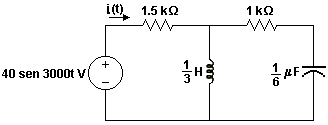
\includegraphics[width=112mm]{book_figures/p026_0.png}
\caption*{Circuit for Problem 026}
\end{figure}

Solution:

The value of the source, $40\sin(3000t)$, can also be expressed as
$40\cos(3000t - 90°)$. Taking this value to a phasor, it is
(40∠$-$90°). We name the three upper nodes, from left to right: 1, 2
and 3. The bottom node is the reference. We name the elements, give
the circuit description and run the simulation with the
\code{sq\char`\\ac} door:

\begin{entry}
sq\ac("e1,1,0,(40∠-90°);r1,1,2,1.5E3;r2,2,3,1E3;l1,2,0,1/3;
      ca,3,0,(1/6)E-6",3000)
\end{entry}

Note that \code{ca} was used as the name of the capacitor, because
the variable \code{c1} is a reserved variable. The direction in
which the elements are defined does not matter in this problem,
except the resistor \code{r1}, which was made to coincide with the
direction of $i(t)$. We start the simulation with \key{ENTER}. We
see on the screen the status messages indicating that the simulation
runs, and then `Done' appears. To see the value of $i(t)$, we can
ask for the value of \code{ir1}, using the \code{absang} tool:

\begin{entry}
sq\absang(ir1)
\end{entry}

\begin{entry}
".015989779∠-126.842333°"
\end{entry}

This is the correct answer. If we wanted to express this current as
a function of time, it would be
$.015989779\cos(3000t - 126.842333°)$.

The \code{thevenin} tool can also make use of alternating current
analysis. Let us see two examples.

\problem{027}

\emph{Problem: If $\omega = 1000$~rad/s, find the input impedance
that would be measured between the terminals: 1) $a$ and $g$; 2) $b$
and $g$; 3) $a$ and $b$.}


% figures added 10 Sep 2026
\begin{figure}[!ht]
\centering
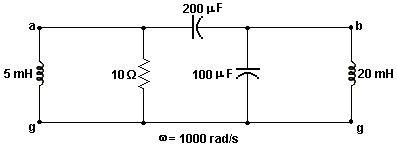
\includegraphics[width=135mm]{book_figures/p027_0.png}
\caption*{Circuit for Problem 027}
\end{figure}

Solution:

We will take the bottom node as the reference, and leave nodes $a$
and $b$ with the same names the drawing has given them. We name the
elements, give the description of the network and execute the
\code{thevenin} tool:

\begin{entry}
sq\thevenin("l1,a,0,5E-3;r1,a,0,10;ca,a,b,200E-6;
            cb,b,0,100E-6;l2,b,0,20E-3",a,0)
\end{entry}

We press \key{ENTER}. We choose Passive as the circuit type and AC
as the analysis type. We press \key{ENTER}. The \code{thevenin} tool
now asks us the value of the radian frequency $\omega$ in rad/s. We
enter 1000, and press \key{ENTER}. We see on the screen the status
messages indicating that one simulation is run. Since we have the
Complex Format mode set to RECTANGULAR, we do not have to use the
\code{→Rect} command to see the answer in rectangular presentation.
For \code{zth} we obtain $2.80898876 + 4.49438202i$ ohms, which is
the correct answer. Let us continue then with the next pair of
nodes:

\begin{entry}
sq\thevenin("l1,a,0,5E-3;r1,a,0,10;ca,a,b,200E-6;
            cb,b,0,100E-6;l2,b,0,20E-3",b,0)
\end{entry}

Note that we only changed node $a$ to node $b$ at the end of the
command. We press \key{ENTER}, choose Passive and AC, press
\key{ENTER}, enter 1000, and press \key{ENTER}. For \code{zth} we
obtain $1.79775281 - 1.1235955i$ ohms, which is the correct answer.
Let us continue:

\begin{entry}
sq\thevenin("l1,a,0,5E-3;r1,a,0,10;ca,a,b,200E-6;
            cb,b,0,100E-6;l2,b,0,20E-3",a,b)
\end{entry}

Again, we only changed the nodes at the end. We press \key{ENTER},
choose Passive and AC, press \key{ENTER}, enter 1000, and press
\key{ENTER}. For \code{zth} we obtain $.112359551 - 3.82022472i$
ohms, which is the correct answer.

\problem{028}

\emph{Problem: If $\omega = 100$~rad/s, find: 1) $Z_{in}$; 2)
$Z_{in}$ if a short circuit is connected from $x$ to $y$.}


% figures added 10 Sep 2026
\begin{figure}[!ht]
\centering
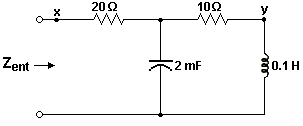
\includegraphics[width=103mm]{book_figures/p028_0.png}
\caption*{Circuit for Problem 028}
\end{figure}

Solution:

We will take the bottom node as the reference, leave nodes $x$ and
$y$ with the names the drawing has given them, and name the middle
node 1. We name the elements, give the description of the network
and execute the \code{thevenin} tool:

\begin{entry}
sq\thevenin("r1,x,1,20;ca,1,0,2E-3;r2,1,y,10;l1,y,0,.1",x,0)
\end{entry}

We press \key{ENTER}. We choose Passive and AC, press \key{ENTER},
enter 100, and press \key{ENTER}. For \code{zth} we obtain
$22. - 6.i$ ohms, which is the correct answer.

For the second part of this problem, the statement asks us to
connect a short circuit between $x$ and $y$. The purpose is to make
one node out of both. For the purposes of the simulation, we could
connect a short circuit between these two nodes. This would add a
new element to the simulation. But we could also do something
better: replace with an $x$ every $y$ that appears in the
description. That way, we will simulate as if $x$ and $y$ were the
same node, which for all practical purposes is equivalent to a short
circuit, since we are not interested in the current through this
short. Not only are we avoiding the addition of a new element, we
are eliminating a node from the circuit:

\begin{entry}
sq\thevenin("r1,x,1,20;ca,1,0,2E-3;r2,1,x,10;l1,x,0,.1",x,0)
\end{entry}

We press \key{ENTER}. We choose Passive and AC, press \key{ENTER},
enter 100, and press \key{ENTER}. For \code{zth} we obtain
$9.6 + 2.8i$ ohms, which is the correct answer.

We have seen in these two examples that the \code{thevenin} tool
also uses alternating current analysis, with success. Let us now see
an example of a circuit in which the inductors and capacitors must
be simulated as impedances, because their values are given to us in
$\Omega$.

\problem{029}

\emph{Problem: Find $I_1$, $I_2$ and $I_3$.}


% figures added 10 Sep 2026
\begin{figure}[!ht]
\centering
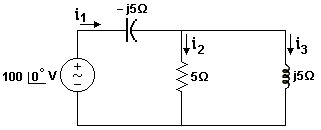
\includegraphics[width=109mm]{book_figures/p029_0.png}
\caption*{Circuit for Problem 029}
\end{figure}

Solution:

The value of the source is already a phasor, and can be reduced from
(100∠0°) to simply 100. The circuit shows three passive elements: a
capacitor, a resistor and an inductor. The values of all of them,
however, have been defined in the circuit as impedances. Therefore,
they must be simulated as impedances. We will take the precaution of
making the numbering and the direction of our impedances coincide
with the currents $I_1$, $I_2$ and $I_3$. With the bottom node as
reference, we name the other nodes and the elements, give the
circuit description and run the simulation. Since we have to give
the program a radian frequency as input data and we do not have any,
we give it any value. I used \code{x}, for example:

\begin{entry}
sq\ac("e1,1,0,100;r1,1,2,-5i;r2,2,0,5;r3,2,0,5i",x)
\end{entry}

Remember that the negative sign must be entered with the negation
key, and not the subtraction key. The imaginary operator $i$ is
entered as indicated in section 6.1. We press \key{ENTER}. We see on
the screen the status messages indicating that the simulation runs,
and then `Done' appears. For the value of $I_1$, with
\code{absang(ir1)} we obtain ``28.2842712∠45.°'' amperes. For the
value of $I_2$, with \code{absang(ir2)} we obtain ``20.∠90.°''
amperes. For the value of $I_3$, with \code{absang(ir3)} we obtain
``20.∠0.°'' amperes. These are the correct answers.

In this problem we have learned that, when a problem presents us
with impedances, it does not matter whether they were obtained from
capacitors or inductors: they must be simulated as impedances.

\section{The separator :}

In the calculator, two separate commands can be joined in a single
line, by means of the separator \code{:} (that is, a colon). For
example, the two commands:

\begin{entry}
sq\ac("e1,1,0,100;r1,1,0,30i",x)
absang(ir1)
\end{entry}

\ldots{}can be joined in a single line, like this:

\begin{entry}
sq\ac("e1,1,0,100;r1,1,0,30i",x):absang(ir1)
\end{entry}

This separator will be used in the following problem.

As we saw in section 6.3, when the frequency is given to us in Hz,
we must first convert it to radians/second to feed it to the
simulator. The following problem illustrates this point, and also
demonstrates that Symbulator handles dependent sources successfully
in alternating current analysis.

\problem{030}

\emph{Problem: Let $V_s = 100∠0°$~V at $f = 50$~Hz in the circuit
shown in the figure. Find the phasor voltage $V_x$, if element X is:
a) a 30~$\Omega$ resistor; b) a 0.5~H inductor; c) a 50~µF
capacitor.}


% figures added 10 Sep 2026
\begin{figure}[!ht]
\centering
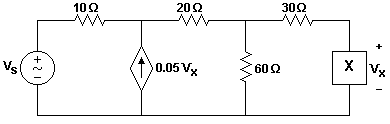
\includegraphics[width=133mm]{book_figures/p030_0.png}
\caption*{Circuit for Problem 030}
\end{figure}

Solution:

From now on, we will round the answers to four figures. Let us run
the first simulation:

\begin{entry}
sq\ac("e1,1,0,100;r1,1,2,10;r2,2,3,20;r3,3,4,30;j1,0,2,.05*v4;
      r4,3,0,60;rx,4,0,30",2*π*50):sq\absang(v4)
\end{entry}

Note that the frequency was not entered in Hz, but converted to
radians/second. Note also the use of the separator \code{:} to join
both commands in one line. We press \key{ENTER}. We see on the
screen the status messages indicating that the simulation runs. When
the simulation finishes, instead of `Done' appearing, the answer to
the last command of the line appears, that is, the voltage
\code{v4}. This is the value of $V_x$: 28.57∠0.° volts (rounded).
This is the correct answer. Let us run the second simulation,
modifying the last element of the description:

\begin{entry}
sq\ac("e1,1,0,100;r1,1,2,10;r2,2,3,20;r3,3,4,30;j1,0,2,.05*v4;
      r4,3,0,60;lx,4,0,.5",2*π*50):sq\absang(v4)
\end{entry}

We press \key{ENTER}. For the value of $V_x$, we obtain
90.24∠25.52° volts, which is the correct answer. Let us run the
third simulation, modifying the last element of the description:

\begin{entry}
sq\ac("e1,1,0,100;r1,1,2,10;r2,2,3,20;r3,3,4,30;j1,0,2,.05*v4;
      r4,3,0,60;cx,4,0,50E-6",2*π*50):sq\absang(v4)
\end{entry}

We press \key{ENTER}. For the value of $V_x$, we obtain
64.71∠$-$49.67° volts, which is the correct answer.

Let us meet two new Symbulator elements, related to magnetic
coupling: mutual inductance and the ideal transformer.

\section{Mutual inductance}

A mutual inductance is a mutual magnetic coupling between two
inductors. It is not a physical ``element'', but it is an element
for the purposes of the simulation.

\subsection{Notation}

In the case of mutual inductance, the minimum information necessary
to describe it completely is the following:

\emph{Identification.} The letter that identifies mutual inductances
is \code{m}.

\emph{Name.} Any name beginning with \code{m} is valid.

\emph{Names of the two coupled inductors.} In Symbulator, a mutual
inductance couples exactly two inductors, each one with a distinct
name. It is necessary to give the simulator the names of the two
inductors that are coupled by the mutual inductance.

It is important that these two inductors coupled by the mutual
inductance be defined in the correct direction. In the circuit
drawing, when two inductors are coupled, a dot is used at one end of
each inductor to indicate the sense of the coupling. So, each
inductor has one end with a dot and the other end without a dot.

When defining these two inductors in Symbulator, their directions
must be defined consistently with the dots. If, when defining the
first inductor, the node that has the dot in the drawing was entered
first, then when defining the second inductor, the first node
defined must also be the one that has the dot in the drawing. Or
vice versa. It is very important to define the nodes of the
inductors in the correct order.

\emph{Value.} For each coupling, there exists a coefficient of
mutual inductance. This coefficient is symbolized by $M$ if its
value is given in henries, and by $k$ if its value is given
dimensionlessly. There is a formula that relates these two
presentations: $k = M/\sqrt{L_1 L_2}$. So, knowing one of them, it
is always possible to know the other. For the purposes of describing
a mutual inductance in Symbulator, the value used is $M$ and it must
be given in henries. Therefore, if the problem gives us the value of
$k$, we must convert it to $M$ before using it in the description.

Take care not to enter the value of a mutual inductance in a unit
other than henries (H). For example, if the value is entered in
millihenries (mH), the answers will be wrong.

So, a mutual inductance is defined as shown below:

\begin{entry}
mname, inductor 1, inductor 2, value in henries
\end{entry}

If necessary, the fifth space is filled with 0.

In direct current analysis, Symbulator ignores mutual inductances.

\subsection{Related answers}

There are no answers related to the mutual inductance itself.
However, each of the two inductors involved will have the related
answers proper to any inductor, which we saw in section 6.9.2.

Let us see some examples.

\problem{031}

\emph{Problem: With the circuit of the figure, present in polar form
the current in the 400~$\Omega$ resistor and the ratio $V_2/V_1$.}


% figures added 10 Sep 2026
\begin{figure}[!ht]
\centering
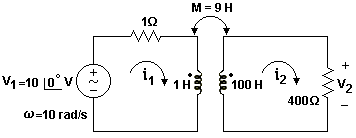
\includegraphics[width=121mm]{book_figures/p031_0.png}
\caption*{Circuit for Problem 031}
\end{figure}

Solution:

We name the nodes from left to right 1, 3 and 2, with the purpose
that \code{v1} and \code{v2} keep in the answers the same names as
in the drawing. Read the circuit description below these lines, and
the comments that follow:

\begin{entry}
sq\ac("e1,1,0,10;r1,1,3,1;l1,3,0,1;l2,2,0,100;r2,2,0,400;
      m1,l1,l2,9",10)
\end{entry}

Note that the first node in the description of each inductor is the
node that has the dot in the drawing. An equally correct alternative
would have been to do the inverse: that the first node in the
description of each inductor had been the node that does not have
the dot in the drawing. The important thing is that the same
convention be used in both inductors. Note that the mutual
inductance does not have to be defined immediately after the
inductors it relates. Note also that the value of the mutual
inductance was entered in henries. We press \key{ENTER}. We see on
the screen the status messages indicating that the simulation runs.
When the simulation finishes, `Done' appears. To find the answers,
we ask for \code{absang(ir2)} and obtain .1724∠$-$16.7° amperes
(rounded), and \code{absang(v2/v1)} and obtain 6.896∠$-$16.7°
(rounded). These are the correct answers.

\problem{032}

\emph{Problem: In the circuit of the figure, find the real average
power absorbed by the source and the two resistors.}


% figures added 10 Sep 2026
\begin{figure}[!ht]
\centering
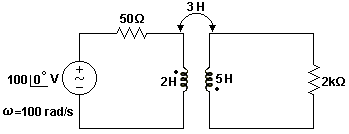
\includegraphics[width=119mm]{book_figures/p032_0.png}
\caption*{Circuit for Problem 032}
\end{figure}

Solution:

Here is the description I used:

\begin{entry}
sq\ac("e1,1,0,100*√2;r1,1,2,50;l1,2,0,2;l2,0,3,5;m1,l1,l2,3;
      r2,3,0,2E3",100)
\end{entry}

Note that the value of the source was converted from its RMS value
to its normal value, directly in the entry field. Note that the
first node in the description of each inductor is the node that has
the dot in the drawing. Note also that the value of the mutual
inductance was entered in henries. We press \key{ENTER}.
We see on the screen the status messages indicating that the
simulation runs. When it finishes, `Done' appears. We are asked for
the real average power absorbed. In alternating current analysis,
the variables in which Symbulator gives us the absorbed power begin
with \code{s}. As theory teaches us, the average power is half the
maximum power. Since we are asked for the real power, we use the
\code{real} command of the calculator. To find the answers, we ask
for \code{real(se1)/2} and obtain $-10.4$ watts; we ask for
\code{real(sr1)/2} and obtain 5.63 watts; we ask for
\code{real(sr2)/2} and obtain 4.77 watts. These are the correct
answers, rounded to three figures.

\problem{033}

\emph{Problem: If $\omega = 100$~rad/s, find the real average power:
a) delivered to the 10~$\Omega$ load, b) to the 20~$\Omega$ load,
and c) delivered by the source.}


% figures added 10 Sep 2026
\begin{figure}[!ht]
\centering
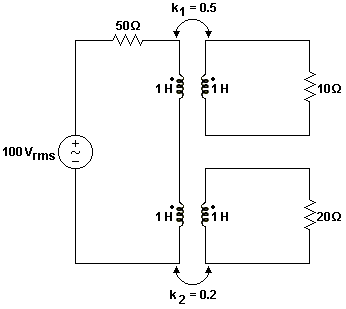
\includegraphics[width=118mm]{book_figures/p033_0.png}
\caption*{Circuit for Problem 033}
\end{figure}

Solution:

Here is the description I used:

\begin{entry}
sq\ac("e1,1,0,100*√2;l1,1,2,1;l2,2,0,1;l3,3,0,1;r1,3,0,10;
      m1,l1,l3,.5*√(1*1);l4,4,0,1;r2,4,0,20;
      m2,l2,l4,.2*√(1*1)",100)
\end{entry}

Note the following:

In a rigorous treatment, in Symbulator, the normal value of the
source must be entered and not its RMS value. For that reason, we
multiply the RMS value by the square root of two, to convert it to
its normal value. It is perfectly valid to do this multiplication
directly in the entry field.

The first node in the description of each inductor is the node that
has the dot in the drawing.

The value of the mutual inductance was converted to henries,
directly in the entry field. Now, this problem is not the best to
illustrate this conversion, because obviously $.5\sqrt{1 \cdot 1}$
is equal to $.5$. Even though placing the conversion is unnecessary
in this problem, in other cases it will not be so. For that reason,
I placed the conversion to illustrate the process.

The circuit of the example is composed of three small circuits.
These three circuits are coupled by mutual inductances. However,
each one of them has a reference node. These three reference nodes
must be node 0. It is necessary that the three share the same
reference node, even though in the drawing the nodes are not
physically connected.

We press \key{ENTER}. We see on the screen the status messages
indicating that the simulation runs. When it finishes, `Done'
appears. As in the previous problem, we are asked for the real
average power absorbed. We ask for \code{real(sr1)/2} and obtain
.842 watts; we ask for \code{real(sr2)/2} and obtain .262 watts; we
ask for \code{real(se1)/2} and obtain $-1.104$ watts. These are the
correct answers (rounded).

\problem{034}

\emph{Problem: Find $I_L$ in the circuit shown.}


% figures added 10 Sep 2026
\begin{figure}[!ht]
\centering
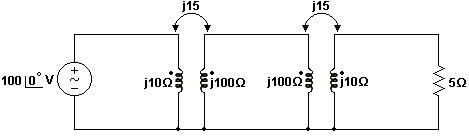
\includegraphics[width=150mm]{book_figures/p034_0.png}
\caption*{Circuit for Problem 034}
\end{figure}

Solution:

This is a very particular problem, and for that reason I saved it
for last. In it, something is presented that Symbulator does not
handle by itself: coupled inductors whose values are given in
$\Omega$. Before solving this problem, we have to take the circuit
to a form that Symbulator can handle. We have two alternatives.

The first alternative is to simulate using impedances. How? By
replacing the mutual inductances with an equivalent made of
impedances. We take advantage of the fact that the coupled inductors
are working as a linear transformer, to replace them with their T
equivalent. For a linear transformer with values $L_1$, $L_2$ and
$M$, the T equivalent is obtained by making a T with elements of
value $L_1 - M$ on one side, $L_2 - M$ on the other side, and $M$ as
the base of the T. In the case of our simulation, this T will be
made with impedances, and there will be no inductors in the circuit.
Below, the description I used to solve the problem with this
alternative. Note that any radian frequency can be used, and any
order of the impedance nodes:

\begin{entry}
sq\ac("e1,1,0,100;r1,1,2,-5i;r2,2,3,85i;rm1,2,0,15i;
      r3,3,4,85i;r4,4,5,-5i;rm2,4,0,15i;rL,5,0,5",x)
\end{entry}

The second alternative is to simulate using inductors. How? Since
the problem has not specified a value for the radian frequency, we
invent any value. I used a unit value: 1~rad/s. Then, I convert all
the values of the inductances and mutual inductances from $\Omega$
to H, using the radian frequency. If the frequency is unity, the
value in ohms will be the same value in henries (without the
imaginary operator, obviously). Below, the description to be used to
solve the problem with this alternative. Note that the order of the
inductor nodes was chosen carefully, to comply with the dot
convention:

\begin{entry}
sq\ac("e1,1,0,100;l1,1,0,10;l2,2,0,100;m1,l1,l2,15;l3,2,0,100;
      l4,3,0,10;m2,l3,l4,15;rL,3,0,5",1)
\end{entry}

In both cases, I called the 5~$\Omega$ resistor \code{rL}. Choose
whichever alternative you prefer. We press \key{ENTER}. We see on
the screen the status messages indicating that the simulation runs.
When it finishes, `Done' appears. We ask for \code{absang(irL)} and
obtain 1.26∠$-$60.2° amperes (rounded), which is the correct answer.

In the previous examples, we have seen how to simulate mutual
inductances in Symbulator, in different types of problems. Let us
now learn about a new element.

\section{Ideal transformer}

An ideal transformer is an idealized model of unity coupling of a
physical transformer. It is assumed to have no losses.

\subsection{Notation}

In the case of the ideal transformer, the minimum information
necessary to describe it completely is the following:

\emph{Identification.} The letter that identifies an ideal
transformer is \code{t}.

\emph{Name.} It must be given any name that begins with \code{t}.

\emph{Nodes.} An ideal transformer has four connection points, two
upper and two lower. For a simulation in Symbulator, the two lower
ones are always assumed connected to the reference node. The upper
ones must each be connected to a distinct node. It is necessary to
give the simulator the names of these two upper nodes to which the
transformer is connected.

\emph{Turns ratio.} An ideal transformer has a turns ratio of one
side with respect to the other. This value must be given to
Symbulator in the form of two numbers, one for each side.

When a transformer has the dots of both sides at the upper nodes, or
both dots at the lower ends, the two numbers of the turns ratio must
have the same sign, for example both positive. On the contrary, when
the transformer has the dot of one side at the upper node but the
dot of the other side at the lower node, the two numbers of the
turns ratio must have opposite signs, for example one positive and
one negative.

So, ideal transformers are defined as shown below:

\begin{entry}
tname, node 1, node 2, turns 1, turns 2
\end{entry}

The description of the ideal transformer always has 5 terms, so
there will never be a need to add a zero at the end.

In direct current analysis, Symbulator ignores ideal transformers.

\subsection{Related answers}

In the case of an ideal transformer, two related answers are given:
the current entering the transformer through the first node, and the
current entering the transformer through the second node. Remember
that these two nodes are the upper ones, since the lower one on both
sides is the reference node. These currents are stored in variables
called \code{inameNODE}, where \code{name} is the name of the ideal
transformer, and \code{NODE} is the name of the node. So, for an
ideal transformer called \code{t1}, connected to nodes 1 and 2, the
related answers will be \code{it11} and \code{it12}. Note that both
currents are considered as entering the transformer through the
upper nodes. Therefore, if one of them is worth, for example, $-5$
amperes, it means that $-5$ amperes are entering, that is, 5 amperes
are leaving.

It is important to note that if either of the ends of the ideal
transformer is an open circuit, both currents will be null.

Let us see some examples.

\problem{035}

\emph{Problem: For the circuit shown, find the RMS value of $I_1$,
$I_2$, $I_3$, and the real average powers consumed in the three
resistors.}


% figures added 10 Sep 2026
\begin{figure}[!ht]
\centering
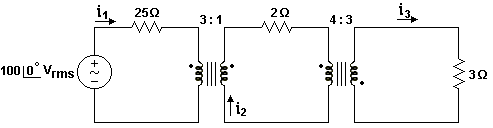
\includegraphics[width=150mm]{book_figures/p035_0.png}
\caption*{Circuit for Problem 035}
\end{figure}

Solution:

Below, the description I used to solve the problem:

\begin{entry}
sq\ac("e1,1,0,100*√2,0;r1,1,2,25,0;t1,2,3,3,1;r2,3,4,2,0;
      t2,4,5,4,-3;r3,5,0,3,0",x)
\end{entry}

Note the following:

The value of the source was converted from RMS value to normal
value.

Any radian frequency can be used.

I filled with zeros the descriptions of those elements whose
descriptions do not have 5 terms. If we forget to do this, we will
get a syntax error.

In the case of transformer \code{t2}, since the dots are one up and
one down, one of the two numbers of the turns ratio in the
description was made negative.

We press \key{ENTER}. We see on the screen the status messages
indicating that the simulation runs. When it finishes, `Done'
appears. To obtain the RMS value of $I_1$, we have three
alternatives: ask for either \code{absang(-ie1/√2)},
\code{absang(ir1/√2)} or \code{absang(it12/√2)}, and we obtain
1.099∠0.° amperes. To obtain the RMS value of $I_2$, we also have
three alternatives: ask for either \code{absang(-it13/√2)},
\code{absang(ir2/√2)} or \code{absang(it24/√2)}, and we obtain
1.30∠0.° amperes. For the RMS value of $I_3$, we have two
alternatives: ask for either \code{absang(-it25/√2)} or
\code{absang(ir3/√2)}, and we obtain 4.40∠180.° amperes.

Remember that Symbulator will always define the two currents of an
ideal transformer as entering the transformer through the two upper
nodes, and the name of each one is \code{i} followed by the name of
the transformer and the name of the node through which the current
enters.

We are asked for the real average power absorbed by the three
resistors. With \code{real(sr1)/2.} we obtain 30.2 watts; with
\code{real(sr2)/2.} we obtain 21.7 watts; and with
\code{real(sr3)/2.} we obtain 58.0 watts. These are the correct
answers (rounded). We used \code{/2.} instead of \code{/2} because
we wished to obtain answers in approximate format.

Let us see two similar problems, but first let us learn some new
concepts about RMS values.

\section{Problems with RMS values}

In two problems that we have seen in this chapter, the value of the
independent source was given to us as an RMS value. As answers, we
were asked for the RMS currents and the average powers. Problems of
this type, using RMS values of voltage and current, and average
powers, are very frequent in alternating current analysis. These
problems can receive two treatments in Symbulator: the rigorous and
the informal.

\subsection{Rigorous treatment}

The two problems we saw before were solved with the rigorous
treatment. This treatment assumes that the values of the independent
sources are entered in normal form, and the voltages, currents and
powers of the answers are also in normal form. Therefore:

When the problem gives us the value of a source in RMS, we must
convert it to normal value when entering it in the description.

If we want the RMS values of the currents and voltages that were
given as answers, we must divide the normal value by the square root
of two to have it in RMS.

If we want the average values of the powers that were given as
answers, we must divide the normal value by two to have it as an
average.

\subsection{Informal treatment}

The two problems that we will see next will be solved with the
informal treatment. This treatment is based on the fact that, if the
values of all the independent sources are entered in RMS, then all
the voltages and currents of the answers will be in RMS, and all the
powers of the answers will be average values. Therefore:

When the problem gives us the value of a source in RMS, we must
enter it as it is. If, on the contrary, it gives it to us as a
normal value, we must convert it to RMS before entering it.

We will receive the currents and voltages of the answers as RMS
values.

We will receive the powers of the answers as average values.

Let us now see two problems, solved with the informal treatment.

\problem{036}

\emph{Problem: For the circuit shown, find the real average powers
consumed in the resistors.}


% figures added 10 Sep 2026
\begin{figure}[!ht]
\centering
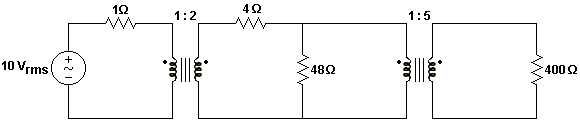
\includegraphics[width=150mm]{book_figures/p036_0.png}
\caption*{Circuit for Problem 036}
\end{figure}

Solution:

Below, the description I used to solve the problem, with the
informal treatment:

\begin{entry}
sq\ac("e1,1,0,10,0;r1,1,2,1,0;t1,2,3,1,2;r2,3,4,4,0;
      r3,4,0,48,0;t2,4,5,1,5;r4,5,0,400,0",x)
\end{entry}

Note that the value of the source was left in RMS. We press
\key{ENTER}. We see on the screen the status messages indicating
that the simulation runs. When it finishes, `Done' appears. We could
obtain the RMS value of any current instantly. However, the problem
does not ask us for any current. We are asked for the real average
power absorbed by the four resistors. Since we are using the
informal method, the powers are already averages. With
\code{real(sr1)} we obtain 4 watts; with \code{real(sr2)} we obtain
4 watts; with \code{real(sr3)} we obtain 3 watts; and with
\code{real(sr4)} we obtain 9 watts. Note that there was no need to
use \code{/2} because the answers were already averages.

\problem{037}

\emph{Problem: For the circuit shown, find the real average powers
consumed by the 10~$\Omega$ resistors. Repeat connecting A and C,
and B and D.}


% figures added 10 Sep 2026
\begin{figure}[!ht]
\centering
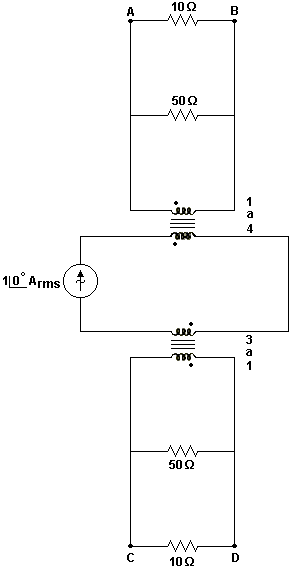
\includegraphics[width=102mm]{book_figures/p037_0.png}
\caption*{Circuit for Problem 037}
\end{figure}

Solution:

Because of the vertical layout of this circuit's drawing, and the
position of the source in it, choosing the reference node for each
section of the circuit could be somewhat complicated. It is
necessary to use the nodes on the right of the circuit (among them B
and D) as the reference in each of the three circuits, because the
two transformers must each have their two lower ends connected to
the reference node. The nodes on the left, from bottom to top, I
named C~$=$~1, 2, 3 and A~$=$~4. Below, the description I used to
solve the first part of the problem, with the informal treatment:

\begin{entry}
sq\ac("r1,1,0,10,0;r2,1,0,50,0;t1,1,2,1,3;j1,2,3,1,0;
      t2,3,4,4,1;r3,4,0,50,0;r4,4,0,10,0",x)
\end{entry}

The value of the source was left in RMS. We press \key{ENTER}. When
the simulation finishes, `Done' appears. The powers are already
averages. With \code{real(sr1)} and \key{$\diamond$} \key{ENTER} we
obtain 62.5 watts; and with \code{real(sr4)} and \key{$\diamond$}
\key{ENTER} we obtain 111.1 watts. Below, the description I used to
solve the second part of the problem, with the informal treatment:

\begin{entry}
sq\ac("r1,1,0,10,0;r2,1,0,50,0;t1,1,2,1,3;j1,2,3,1,0;
      t2,3,1,4,1;r3,1,0,50,0;r4,1,0,10,0",x)
\end{entry}

Note that I did not use a short circuit to connect A with C, but
instead replaced node 4 with node 1 in the description. There is no
need to connect B with D, because both are the reference node. We
press \key{ENTER}. When the simulation finishes, `Done' appears.
With \code{real(sr1)} and \key{$\diamond$} \key{ENTER} we obtain
1.736 watts; and with \code{real(sr4)} and \key{$\diamond$}
\key{ENTER} we obtain the same value as \code{sr1}.

We have seen in these two problems the way in which the values of
the sources in RMS can be used, with the informal treatment, to
obtain answers directly in RMS, and the powers as averages.

Let us see a final example, of the \code{thevenin} tool applied to a
circuit with ideal transformers.

\problem{038}

\emph{Problem: Find the Th\'evenin equivalent at terminals $a$ and
$b$ for the network shown in the figure.}


% figures added 10 Sep 2026
\begin{figure}[!ht]
\centering
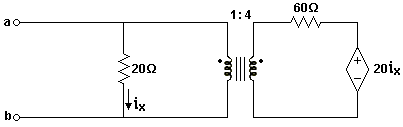
\includegraphics[width=137mm]{book_figures/p038_0.png}
\caption*{Circuit for Problem 038}
\end{figure}

Solution:

Below, the description:

\begin{entry}
sq\thevenin("rx,a,0,20,0;t1,a,1,1,4;r1,1,2,60,0;
            e1,2,0,20*irx,0",a,0)
\end{entry}

We press \key{ENTER}. We choose Passive and AC, and press
\key{ENTER}. We enter \code{x}, or any other value, as the radian
frequency and press \key{ENTER}. For \code{zth} we obtain 4 ohms,
which is the correct value.

With this example, we have finished the chapter on numerical
simulation of alternating current.
